
\subsubsection{【概要】}
hiki2latexのtable処理部

\subsubsection{【仕様】}\begin{itemize}
\item hiki記法の表をtabularへ変換
\item 連結作用素に対応
\item 行連結では中心に表示を移動
\item 縦罫は基本使わない
\item 横罫はheader内枠と上下外枠のみ
\end{itemize}
\subsubsection{【hiki】}\begin{quote}\begin{verbatim}
||>A11||>A12||
||^^A21||A22||>A23||
||A11||^A22||A12||
||A21||A23||
\end{verbatim}\end{quote}
\begin{table}[htbp]\begin{center}
\caption{}
\begin{tabular}{lllll}
\hline
\multicolumn{2}{l}{A11 }  &\multicolumn{2}{l}{A12 }  \\ \hline
 &A22  &\multicolumn{2}{l}{A23 }  \\
A21  &A11  &A22  &A12  \\
 &A21  & &A23  \\
\hline
\end{tabular}
\label{default}
\end{center}\end{table}
%for inserting separate lines, use \hline, \cline{2-3} etc.

\subsubsection{【latex】}\begin{lstlisting}[style=]
¥begin{center}¥begin{table}[htbp]¥begin{tabular}{ccccc}
¥hline
¥multicolumn{2}{c}{A11 }  &¥multicolumn{2}{c}{A12 }  &  ¥¥ ¥hline
 &A22  &¥multicolumn{2}{c}{A23 }  &  ¥¥
A21  &A11  &A22  &A12  &  ¥¥
 &A21  & &A23  &  ¥¥
¥hline
¥end{tabular}¥end{table}¥end{center}
%横罫を入れる場合は, ¥hline, ¥cline{2-3}などで.
\end{lstlisting}
\begin{figure}[htbp]\begin{center}
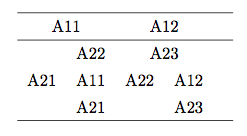
\includegraphics[width=6cm]{./table.png}
\caption{}
\label{default}\end{center}\end{figure}
\subsubsection{【コード解説】}
元のHTMLOutputではそれぞれの要素で対応していたが,LatexOutputではtable\_closeにて
\begin{lstlisting}[style=customRuby]
    def table_close
      @f << make_table
    end
\end{lstlisting}
としている.make\_tableは下請けにmake\_matrixを読んでおり,ここでほぼ全ての作業をしている.作業内容は
\begin{itemize}
\item matrixを作る
\item 縦連結を処理\begin{itemize}
\item 縦連結の数(rs)だけ下行に追加
\item 連結の中心(c\_rs)に内容を表記
\end{itemize}
\item 横連結をmulticolumnで処理\begin{itemize}
\item ついでに最大列数(max\_col)を記録
\end{itemize}
\end{itemize}\begin{lstlisting}[style=customRuby]
bob% cat table.rb
cont = File.readlines("table")

cont.each{|line|
  p tmp=line.split('||')
}

t_matrix=[]
cont.each{|line|
  tmp=line.split('||')
  tmp.slice!(0)
  tmp.slice!(-1) if tmp.slice(-1)=="\n"
  tmp.each_with_index{|ele,i| tmp[i] = ele.match(/\s*(.+)/)[1]}
  t_matrix << tmp
}

t_matrix.each_with_index{|line,i|
  line.each_with_index{|ele,j|
    if ele=~/\^+/ then
      t_matrix[i][j]=""
      rs=$&.size
      c_rs=rs/2
      rs.times{|k| t_matrix[i+k+1].insert(j,"")}
      t_matrix[i+c_rs][j]=$'
    end
  }
}
p t_matrix

max_col=0
t_matrix.each_with_index{|line,i|
  n_col=line.size
  line.each_with_index{|ele,j|
    if ele=~/>+/ then
      cs=$&.size
      t_matrix[i][j]= "\\multicolumn{#{cs+1}}{c}{#{$'}} "
      n_col+=cs
    end
  }
  max_col = n_col if n_col>max_col
}
p t_matrix
p max_col
\end{lstlisting}
